\section{Benutzungsoberfläche}


\subsection{Startfenster}

\begin{figure}[hp] 
  \centering
     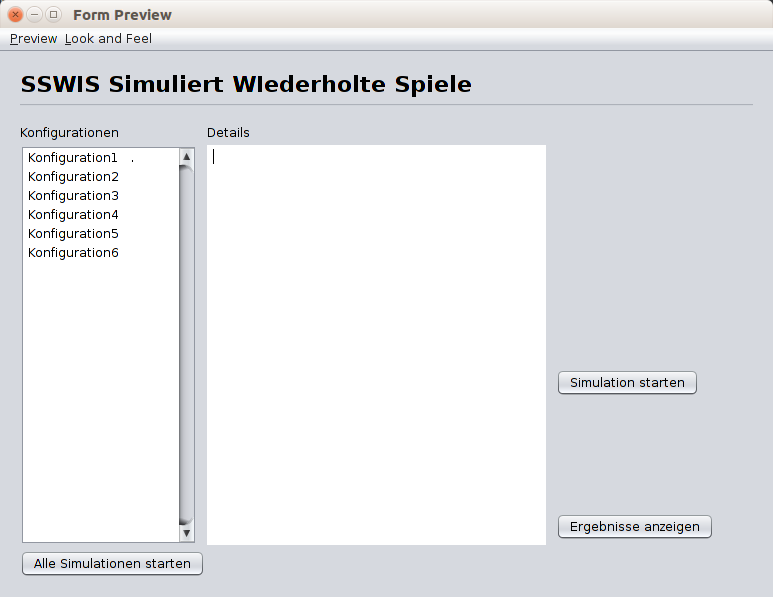
\includegraphics[width=1.1\textwidth]{GUI_Entwurf/Startfenster.png}
  \caption{Hauptfenster}
  \label{fig:Bild1}
\end{figure}

\begin{description}


\item[1. Menü Stufenspiele] Enthält den Menüpunkt 'Stufenspiele verwalten'. Dieser führt zur Stufenspiel Verwaltung.

\item[2. Menü Strategien] Enthält den Menüpunkt 'Kombinierte Strategien verwalten'. Dieser führt zu dem Kombinierte Strategien Verwaltung.

\item[3. Menü Initialisierungen] Enthält Menüpunkt 'Initialisierungen bearbeiten' und 'Neue Initialisierung'. 'Initialisierungen bearbeiten' öffnet ein OpenFileDialog in dem Initialisierungen gelöscht, umbenannt und in das Initialisierungsfenster geöffnet und bearbeitet werden können. 'Neue Initialisierung' öffnet das Initialisierungs-Fenster.

\item[4. Menü Konfigurationen] Enthält Menüpunkt 'Neue Konfiguration'. Dieser öffnet das Konfigurations-Fenster.

\item[5. Menü Ergebnisse] Enthält Menüpunkt 'Ergebnisse vergleichen'. Dieser öffnet das Vergleichfenster.

\item[6. Liste der Konfigurationen] Diese zeigt die Liste der erstellten Konfigurationen an. Werden neue Konfigurationen erstellt, werden dievorigen Konfigurationen durch die Neuen in der Liste ersetzt.

\item[7. Details] Ist eine Konfiguration in der Liste ausgewählt, werden hier die Parameter der Konfiguration angezeigt.

\item[8. Simulation starten] Ist eine Konfiguration in der Liste ausgewählt, ist dieser Button aktiviert. Nach dem betätigen wird in einem Pop-Up-Fenster die Anzahl der Wiederholungen abgefragt. Danach wird die Simulation gestartet.

\item[9. Ergebnisse anzeigen] Wurde eine Simulation mit der in der Liste ausgewählten Konfiguration durchgeführt, ist dieser Button aktiviert. Er öffnet das Ergebnisfenster mit den Ergebnissen, der letzten Durchführung.

\item[10. Alle Simulationen starten] Nach dem betätigen wird in einem Pop-Up-Fenster die Anzahl der Wiederholungen abgefragt. Danach werrden die Simulationen für alle Konfigurationen in der Liste gestartet.

\end{description}

\pagebreak

\subsection{Stufenspiele Verwaltung}

\begin{figure}[hp] 
  \centering
     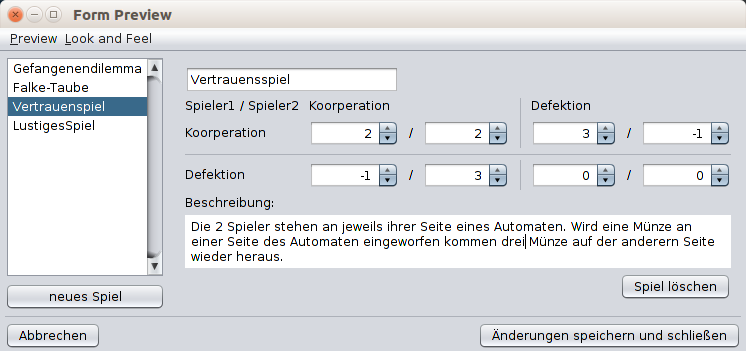
\includegraphics[width=1.1\textwidth]{GUI_Entwurf/SpieleMenue.png}
  \caption{Stufenspiel Verwaltung}
  \label{fig:Bild1}
\end{figure}

\begin{description}

\item[1. Liste] Zeigt alle zuvor gespeicherten die voreingestellten Stufenspiele. Wird ein Spiel ausgewählt erscheinen alle Parameter in den Feldern zwei bis vier rechts neben der Liste.

\item[2. Name] Der Name des Stufenspiels lässt sich bearbeiten.

\item[3. Auszahlungen] Alle acht Felder für die Auszahlung, lassen sich bearbeiten.

\item[4. Beschreibung] Es lässt sich eine Beschreibung für das Spiel angeben.

\item[5. neues Spiel] Fügt ein neues Stufenspiel in die Liste an. 

\item[6. Spiel löschen] Das in der Liste ausgewählte Spiel wird gelöscht.

\item[7. Abbrechen] Alle zuvor vorgenommen Änderungen inklusive das Erstellen neuer Spiele werden verworfen und die Spiele Verwaltung schließt sich.

\item[8. Änderungen speichern und schließen] Alle zuvor vorgenommen Änderungen werden gespeichert und die Spiele Verwaltung schließt sich.

\end{description}

\pagebreak

\subsection{Kombinierte Strategien Verwaltung}


\begin{figure}[hp]
  \centering
     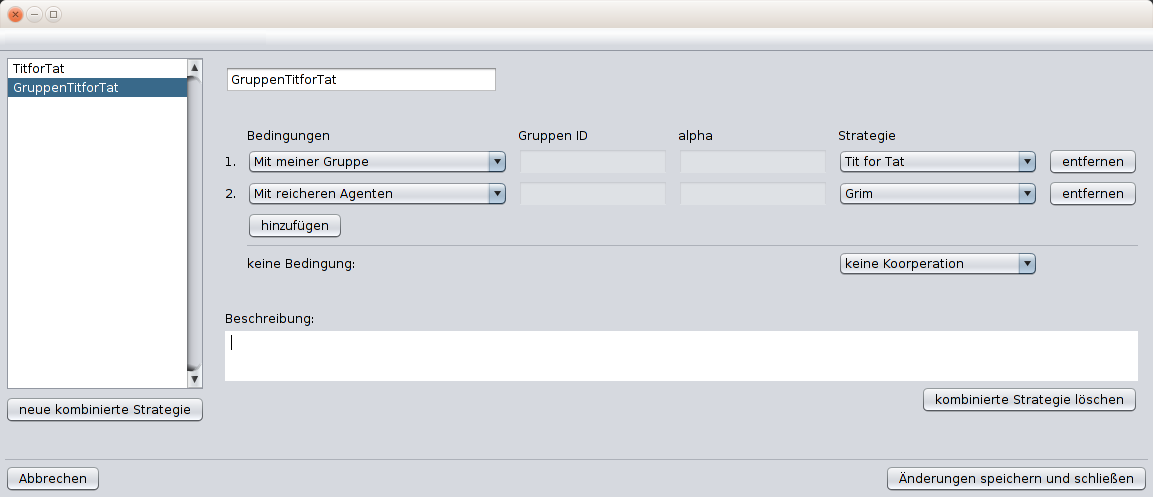
\includegraphics[width=1.15\textwidth]{GUI_Entwurf/StrategienMenue.png}
  \caption{Kombinierte Strategien Verwaltung}
  \label{fig:Bild1}
\end{figure}

\begin{description}

\item[1. Liste] Zeigt alle zuvor gespeicherten  kombinierten Strategien. Wird ein kombinierte Strategie ausgewählt, erscheinen alle Parameter in den Feldern zwei bis elf rechts neben der Liste.

\item[2. Name] Der Name der kombinierten Strategie kann geändert werden.

\item[3. Nummerierung] Gibt die Reihenfolge an nach denen Bedingungen geprüft werden.

\item[4. Bedingung] Bedingung mit der die rechten Strategie gewählt wird.

\item[5. Gruppen ID] Ist aktiviert wenn Bedingung 'mit Gruppe \textit{Gruppen ID}' ausgewählt ist. Hier kann die entsprechende ID der Gruppe eingegeben werden.

\item[6. alpha] Ist aktiviert wenn Bedingung 'mit Wahrscheinlichkeit \textit{Gruppen alpha}' ausgewählt ist. Hier kann die entsprechende Wahrscheinlichkeit eingegeben werden.

\item[7. Strategie] Die Strategie, die eintreten soll wenn die Bedingung links daneben erfüllt ist.

\item[8. entfernen] Entfernt diese Zeile mit den entsprechenden Feldern drei bis sieben. Die Nummerierung wird entsprechend angepasst.

\item[9. hinzufügen] 

\item[10. keine Bedingung] 

\item[11. Beschreibung] 

\item[12. neue kombinierte Strategie] 

\item[13. kombinierte Strategie löschen] 

\item[14. Abbrechen] 

\item[15. Änderungen speichern und schließen] 

\end{description}

\pagebreak

\subsection{Initialisierung erstellen}

\begin{figure}[hp] 
  \centering
     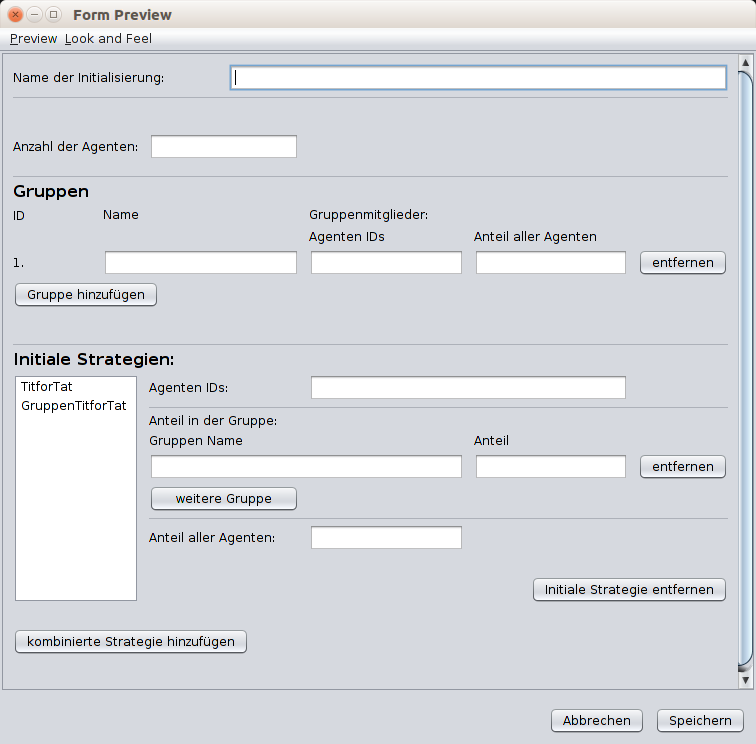
\includegraphics[width=1.1\textwidth]{GUI_Entwurf/NeueInitialisierung.png}
  \caption{Initialisierung}
  \label{fig:Bild1}
\end{figure}


\begin{description}

\item[1. Name] 

\item[2. Anzahl der Agenten] 

\item[3. Gruppen - ID] 

\item[4. Gruppen - Name] 

\item[5. Gruppen - AgentenIDs] 

\item[6. Gruppen - Anteil aller Agenten] 

\item[7. Gruppen - entfernen] 

\item[8. Gruppen - Gruppe hinzufügen] 

\item[9. Initiale Strategien - Liste] 

\item[10. Initiale Strategien - Agenten IDs] 

\item[11. Initiale Strategien - Gruppen Name] 

\item[12. Initiale Strategien - Anteil] 

\item[13. Initiale Strategien - entfernen] 

\item[14. Initiale Strategien - weitere Gruppe] 

\item[15. Initiale Strategien - Anteil der Agenten] 

\item[16. Initiale Strategien - kombinierte Strategie hinzufügen] 

\item[17. Abbrechen] 

\item[18. Speichern] 

\end{description}


\pagebreak

\subsection{Konfigurationen erstellen}

\begin{figure}[hp] 
  \centering
     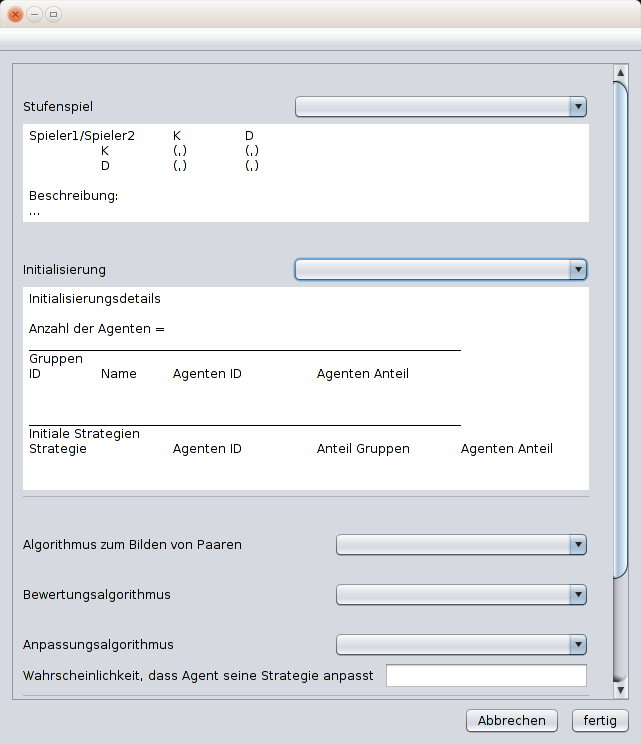
\includegraphics[width=1.0\textwidth]{GUI_Entwurf/NeueKonfiguration1.png}
  \caption{Konfiguration}
  \label{fig:Bild2}
\end{figure}

\begin{figure}[hp] 
  \centering
     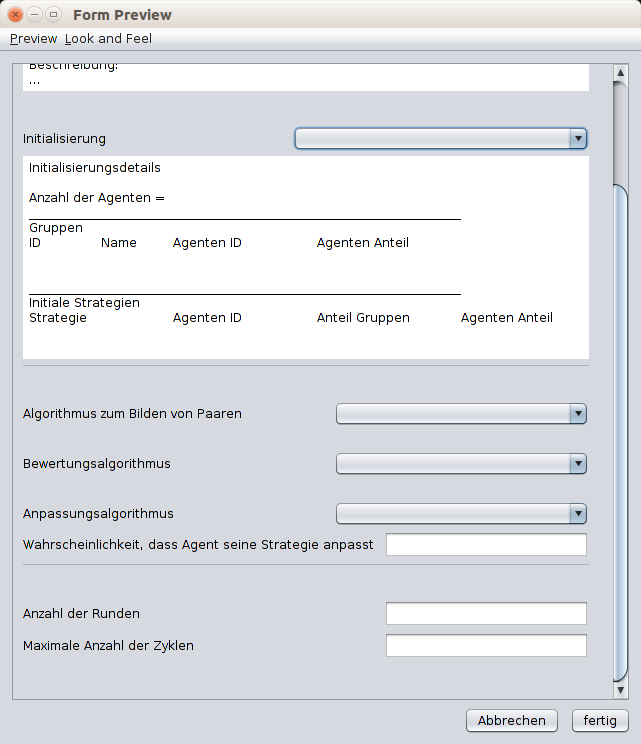
\includegraphics[width=1.0\textwidth]{GUI_Entwurf/NeueKonfiguration2.png}
  \caption{Konfiguration}
  \label{fig:Bild2}
\end{figure}

\begin{description}

\item[1. Stufenspiel] 

\item[2. Initialisierung] 

\item[3. Algorithmus zum Bilden von Paaren] 

\item[4. Bewertungsalgorithmus] 

\item[5. Anpassungsalgorithmus] 

\item[6. Wahrscheinlichkeit für Strategieanpassung] 

\item[7. Anzahl der Runden] 

\item[8. Maximale Anzahl der Zyklen] 

\item[9. fertig] 

\item[10. Abbrechen]


\end{description}

\pagebreak


\subsection{Ergebnisse anzeigen}

\begin{figure}[hp] 
  \centering
     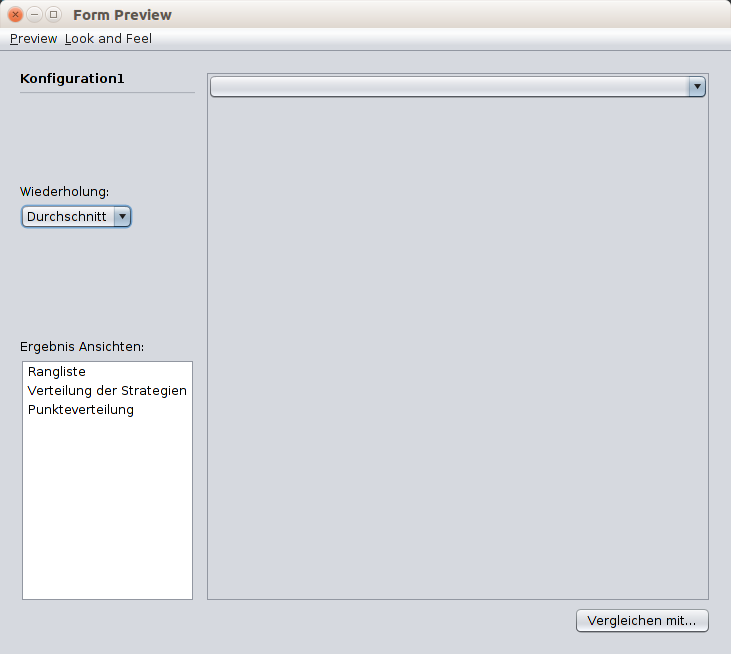
\includegraphics[width=1.1\textwidth]{GUI_Entwurf/Ergebnisfenster(1).png}
  \caption{Ergebnisfenster}
  \label{fig:Bild7}
\end{figure}

\begin{description}

\item[1. Konfiguration] 

\item[2. Wiederholung] 

\item[3. Liste Ergebnis Ansichten] 

\item[4. Ansicht] 

\item[5. Ansicht Optionen] 

\item[6. Vergleichen mit...] 

\end{description}

\pagebreak


\subsection{Ergebnisse vergleichen}

\begin{figure}[hp] 
  \centering
     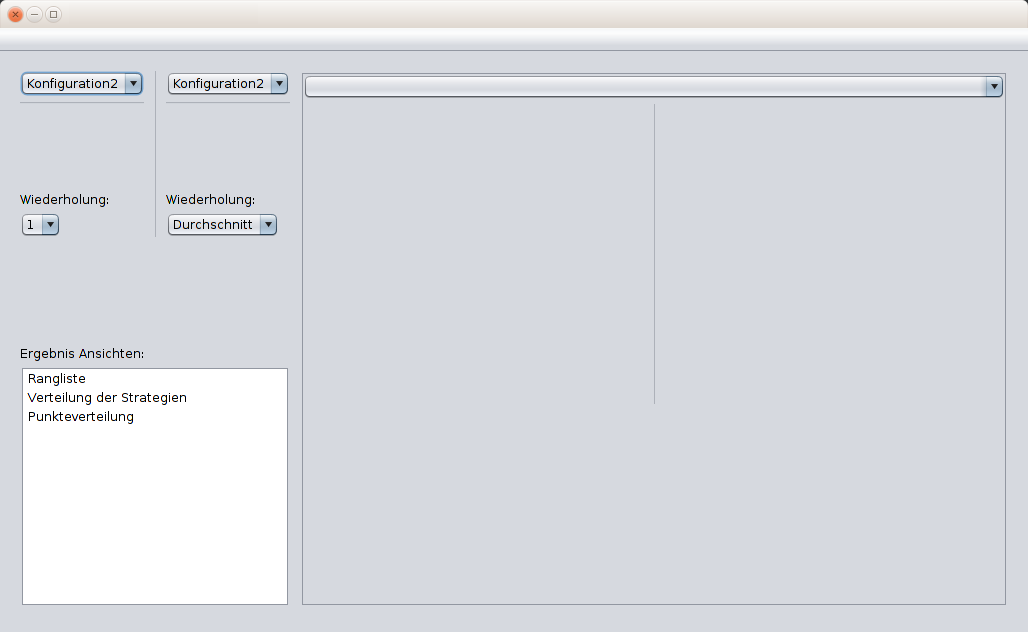
\includegraphics[width=1.15\textwidth]{GUI_Entwurf/Vergleichfenster.png}
  \caption{Vergleichenfenster}
  \label{fig:Bild1}
\end{figure}

\begin{description}

\item[1. Konfiguration] 

\item[2. Wiederholung] 

\item[3. Liste Ergebnis Ansichten] 

\item[4. Ansicht] 

\item[5. Ansicht Optionen] 

\end{description}



